\chapter{Wasserstein 空間と測地線・曲率}
\label{ch:seminar-03}

\begin{remark}{本章の設定}{sem-ch4-setup}
  本章では $(\X, d)$ を完備可分な距離空間（Polish 空間，
  定義~\ref{def:sem-polish}）とし，$p \geq 1$ を固定する．
  $\X$ 上の確率測度全体を $\Mm_+^1(\X)$ と書き
  （第~\ref{ch:seminar-01}~章の定義~\ref{def:sem-kantorovich} の Kantorovich 問題
  はこの設定の下で導入されている），
  本章では特に\textbf{$p$ 次モーメントが有限な}測度の空間
  \[
    \Pp_p(\X) \defeq
    \left\{ \alpha \in \Mm_+^1(\X) \;\middle|\;
    \int_{\X} d(x, x_0)^p \, \d\alpha(x) < \infty
    \text{ for some } x_0 \in \X \right\}
  \]
  を主舞台とする．条件は固定点 $x_0$ の取り方によらないことが
  三角不等式 $d(x, x_0) \leq d(x, x_0') + d(x_0', x_0)$ から従う．

  ユークリッド設定 $\X = \R^n$ では距離 $d(x, y) = \norm{x - y}_2$ と
  ルベーグ測度 $\Lcal^n$ を既定とする．
  本章で必要となる Riemann 多様体・条件付き分布・Brenier の定理などの
  外部知見は，必要箇所で参照のみを記し，証明は対応文献に委ねる．
\end{remark}

%% ============================================================
%% §1 Wasserstein 距離
%% ============================================================
\section{Wasserstein 距離}
\label{sec:sem-wasserstein}

Kantorovich 問題（定義~\ref{def:sem-kantorovich}）はコスト関数
$c \colon \X \times \Y \to \R_+$ を任意に取れる枠組みであった．
本節ではコストを基底距離 $d$ の $p$ 乗 $c(x, y) = d(x, y)^p$ に特殊化する．
このとき得られる最適値は，確率測度の空間に\textbf{距離}を与え，
さらに次節以降で見るように\textbf{幾何構造}までを誘導する．

\subsection{定義}

\begin{definition}{$p$-Wasserstein 距離}{sem-wasserstein}
  $(\X, d)$ を距離空間，$p \geq 1$ とする．
  確率測度 $\alpha, \beta \in \Mm_+^1(\X)$ に対し，
  コスト $c(x, y) = d(x, y)^p$ の Kantorovich 問題
  （定義~\ref{def:sem-kantorovich}）の最適値の $1/p$ 乗
  \[
    \Wass_p(\alpha, \beta) \defeq
    \MK_{d^p}(\alpha, \beta)^{1/p}
    = \left( \inf_{\pi \in \Couplings(\alpha, \beta)}
      \int_{\X \times \X} d(x, y)^p \, \d\pi(x, y) \right)^{1/p}
  \]
  を $\alpha, \beta$ 間の\textbf{$p$-Wasserstein 距離}という．
  ヒストグラム $\mathbf{a} \in \R_+^n$, $\mathbf{b} \in \R_+^m$ と
  距離行列 $\distD \in \R_+^{n \times m}$（$D_{i,j} = d(x_i, y_j)$）に対する
  離散版は
  \[
    \WassD_p(\mathbf{a}, \mathbf{b})
    \defeq \MKD_{\distD^{\circ p}}(\mathbf{a}, \mathbf{b})^{1/p}
  \]
  で与えられる（$\distD^{\circ p}$ は成分ごとの $p$ 乗 $D_{i,j}^p$）．
\end{definition}

\begin{example}{Dirac 測度間の Wasserstein 距離}{sem-wass-dirac}
  $x, y \in \X$ に対する 2 つの Dirac 測度 $\delta_x, \delta_y$ について，
  $\Couplings(\delta_x, \delta_y) = \{\delta_{(x, y)}\}$ のみであるから
  \[
    \Wass_p(\delta_x, \delta_y)
    = \left( \int_{\X \times \X} d(u, v)^p \, \d\delta_{(x, y)}(u, v) \right)^{1/p}
    = d(x, y).
  \]
  すなわち埋め込み $\X \hookrightarrow \Pp_p(\X),\; x \mapsto \delta_x$ は
  距離を保つ（等長埋め込みである）．
  Wasserstein 距離は\textbf{基底空間の距離 $d$ を測度空間に自然に持ち上げる}．
\end{example}

\subsection{距離性}

定義からは $\Wass_p$ が「距離」と呼ぶに値することは明らかでない．
正値性・対称性は定義から比較的すぐ従うが，
三角不等式は基底空間の三角不等式と Minkowski 不等式を
\textbf{1 つの確率測度の上で}結合する仕掛けが必要である．
そのための補助命題が次の Gluing lemma である．

\begin{theorem}{$\Wass_p$ は $\Pp_p(\X)$ 上の距離である}{sem-wass-metric}
  $(\X, d)$ を Polish 距離空間，$p \geq 1$ とする．
  $\Wass_p$ は $\Pp_p(\X)$ 上で距離の公理を満たす：
  \begin{enumerate}
    \item[\textup{(i)}]
      $\Wass_p(\alpha, \beta) \geq 0$ かつ
      $\Wass_p(\alpha, \beta) = 0 \iff \alpha = \beta$，
    \item[\textup{(ii)}]
      $\Wass_p(\alpha, \beta) = \Wass_p(\beta, \alpha)$，
    \item[\textup{(iii)}]
      $\Wass_p(\alpha, \gamma) \leq \Wass_p(\alpha, \beta) + \Wass_p(\beta, \gamma)$．
  \end{enumerate}
\end{theorem}

\begin{proposition}{Gluing lemma}{sem-gluing}
  $\X, \Y, \Z$ を Polish 距離空間とし，
  $\pi_1 \in \Couplings(\alpha, \beta) \subset \Mm_+^1(\X \times \Y)$，
  $\pi_2 \in \Couplings(\beta, \gamma) \subset \Mm_+^1(\Y \times \Z)$
  が与えられているとする（$\pi_1, \pi_2$ は中間の周辺 $\beta \in \Mm_+^1(\Y)$ を共有）．
  このとき，$\X \times \Y \times \Z$ 上の確率測度 $\mu$ で，
  \[
    (P_{\X \times \Y})\pushforward \mu = \pi_1,
    \qquad
    (P_{\Y \times \Z})\pushforward \mu = \pi_2
  \]
  を満たすものが存在する．
\end{proposition}

\begin{proof}
  Polish 空間上の確率測度は\textbf{正則条件付き確率}の存在が保証される
  （Disintegration theorem）．これにより
  $\pi_1$ の $y \in \Y$ に関する条件付き分布 $\pi_1(\cdot \mid y) \in \Mm_+^1(\X)$，
  $\pi_2$ の $y \in \Y$ に関する条件付き分布 $\pi_2(\cdot \mid y) \in \Mm_+^1(\Z)$
  がとれて
  \[
    \d\pi_1(x, y) = \d\pi_1(x \mid y) \, \d\beta(y),
    \qquad
    \d\pi_2(y, z) = \d\pi_2(z \mid y) \, \d\beta(y)
  \]
  と書ける．これらを用いて $\X \times \Y \times \Z$ 上の測度
  \[
    \d\mu(x, y, z) \defeq \d\pi_1(x \mid y) \, \d\beta(y) \, \d\pi_2(z \mid y)
  \]
  を定める．構成より
  \[
    (P_{\X \times \Y})\pushforward \mu(\d x, \d y)
    = \d\pi_1(x \mid y) \, \d\beta(y)
    = \d\pi_1(x, y),
  \]
  \[
    (P_{\Y \times \Z})\pushforward \mu(\d y, \d z)
    = \d\beta(y) \, \d\pi_2(z \mid y)
    = \d\pi_2(y, z).
  \]
  したがって $\mu$ は所望の周辺条件を満たす．
\end{proof}

\begin{figure}[H]
\centering
\begin{tikzpicture}[scale=1.0]
  %% 中央：3 次元的な箱（X × Y × Z）の概念表現
  \node[font=\small] at (0, 3.6) {$\mu \in \Mm_+^1(\X \times \Y \times \Z)$};
  \draw[thick] (-1.4, 1.8) -- (1.4, 1.8) -- (1.4, 3.2) -- (-1.4, 3.2) -- cycle;
  \draw[thick] (1.4, 1.8) -- (2.0, 2.4) -- (2.0, 3.8) -- (1.4, 3.2);
  \draw[thick] (-1.4, 3.2) -- (-0.8, 3.8) -- (2.0, 3.8);
  \draw[dashed, gray] (-1.4, 1.8) -- (-0.8, 2.4) -- (2.0, 2.4);
  \draw[dashed, gray] (-0.8, 2.4) -- (-0.8, 3.8);
  %% 中央の濃淡で μ の存在を示唆
  \fill[purple!40, opacity=0.6] (-0.3, 2.4) ellipse (0.3 and 0.2);
  \fill[purple!60, opacity=0.7] (0.6, 2.7) ellipse (0.4 and 0.25);

  %% 左下：π_1 ∈ M^1_+(X × Y)
  \draw[thick] (-5.2, -1.0) rectangle (-2.4, 0.6);
  \node[font=\small, below] at (-3.8, -1.1) {$\pi_1 \in \Couplings(\alpha, \beta)$};
  \node[font=\footnotesize, below right] at (-2.4, -1.0) {$\X$};
  \node[font=\footnotesize, above left] at (-5.2, 0.6) {$\Y$};
  \fill[blue!50, opacity=0.7] (-4.5, -0.3) ellipse (0.4 and 0.3);
  \fill[blue!50, opacity=0.7] (-3.0, 0.1) ellipse (0.5 and 0.3);

  %% 右下：π_2 ∈ M^1_+(Y × Z)
  \draw[thick] (2.4, -1.0) rectangle (5.2, 0.6);
  \node[font=\small, below] at (3.8, -1.1) {$\pi_2 \in \Couplings(\beta, \gamma)$};
  \node[font=\footnotesize, below right] at (5.2, -1.0) {$\Z$};
  \node[font=\footnotesize, above left] at (2.4, 0.6) {$\Y$};
  \fill[red!50, opacity=0.7] (3.1, -0.3) ellipse (0.4 and 0.3);
  \fill[red!50, opacity=0.7] (4.6, 0.1) ellipse (0.5 and 0.3);

  %% 上下：(X × Z)-射影
  \draw[thick] (-1.6, -2.6) rectangle (1.6, -1.4);
  \node[font=\small, below] at (0, -2.7)
    {$(P_{\X \times \Z})\pushforward \mu \in \Couplings(\alpha, \gamma)$};
  \fill[purple!60, opacity=0.7] (-0.7, -2.0) ellipse (0.3 and 0.2);
  \fill[purple!60, opacity=0.7] (0.6, -1.8) ellipse (0.4 and 0.25);

  %% 矢印：μ → π_1, μ → π_2, μ → (X × Z)-周辺
  \draw[->, thick, gray] (-1.5, 2.2) to[bend right=18] (-2.5, -0.2)
    node[midway, above left, font=\footnotesize, gray]
    {$P_{\X \times \Y}\!\pushforward$};
  \draw[->, thick, gray] (1.5, 2.2) to[bend left=18] (2.5, -0.2)
    node[midway, above right, font=\footnotesize, gray]
    {$P_{\Y \times \Z}\!\pushforward$};
  \draw[->, thick, gray] (0, 1.7) -- (0, -1.3)
    node[midway, right, font=\footnotesize, gray]
    {$P_{\X \times \Z}\!\pushforward$};
\end{tikzpicture}
\caption{Gluing lemma の概念図．与えられた 2 つのカップリング
$\pi_1 \in \Couplings(\alpha, \beta)$ と $\pi_2 \in \Couplings(\beta, \gamma)$
を「$\Y$ の上で同じ条件付き分布構造を共有する」ように貼り合わせ，
3 因子上の測度 $\mu$ を構成する．副産物として $(P_{\X \times \Z})\pushforward \mu$
は $\alpha$ と $\gamma$ の新しいカップリングを与える．}
\label{fig:sem-gluing}
\end{figure}

\begin{proof}[定理~\ref{thm:sem-wass-metric} の証明]
  \textbf{(i) 正値性・同一性．}
  カップリング上で $d(x, y)^p \geq 0$ ゆえ $\Wass_p \geq 0$．
  $\alpha = \beta$ ならば対角カップリング
  $(\Id, \Id)\pushforward \alpha \in \Couplings(\alpha, \alpha)$ をとると
  $\int d(x, y)^p \, \d\pi = \int d(x, x)^p \, \d\alpha = 0$ より
  $\Wass_p(\alpha, \alpha) = 0$．
  逆に $\Wass_p(\alpha, \beta) = 0$ ならば，下限を達成する最適カップリング
  $\pi^* \in \Couplings(\alpha, \beta)$ が存在し（連続版でも Polish の下では
  Prokhorov の定理と $d^p$ の下半連続性により存在する），
  $\int d(x, y)^p \, \d\pi^* = 0$ から $\pi^*$ は対角集合
  $\{(x, y) \in \X \times \X \mid x = y\}$ 上に集中する．
  両周辺をとると $\alpha = (P_1)\pushforward \pi^* = (P_2)\pushforward \pi^* = \beta$．

  \textbf{(ii) 対称性．}
  座標入れ替え $S(x, y) = (y, x)$ による押し出しは
  $\Couplings(\alpha, \beta)$ と $\Couplings(\beta, \alpha)$ の間の
  全単射を与える．$d(x, y)^p = d(y, x)^p$ ゆえ
  $\int d^p \, \d\pi = \int d^p \, \d(S\pushforward \pi)$ となり，
  下限値が等しい．

  \textbf{(iii) 三角不等式．}
  $\alpha, \beta, \gamma \in \Pp_p(\X)$ を任意に取る．
  最適カップリング $\pi_1 \in \Couplings(\alpha, \beta)$，
  $\pi_2 \in \Couplings(\beta, \gamma)$ をとり
  （上述の通り存在する），命題~\ref{prop:sem-gluing}
  により $\X \times \X \times \X$ 上の測度 $\mu$ で周辺が
  $\pi_1, \pi_2$ に一致するものを構成する．
  射影 $P_{1,3}(x, y, z) = (x, z)$ による押し出し
  $(P_{1,3})\pushforward \mu \in \Couplings(\alpha, \gamma)$
  を $\Wass_p(\alpha, \gamma)$ の評価に用いると，
  距離の三角不等式 $d(x, z) \leq d(x, y) + d(y, z)$ と
  $L^p(\mu)$ における Minkowski 不等式から
  \begin{align*}
    \Wass_p(\alpha, \gamma)
    &\leq \left( \int_{\X^3} d(x, z)^p \, \d\mu(x, y, z) \right)^{1/p} \\
    &\leq \left( \int_{\X^3} \bigl( d(x, y) + d(y, z) \bigr)^p \, \d\mu \right)^{1/p} \\
    &\leq \left( \int_{\X^3} d(x, y)^p \, \d\mu \right)^{1/p}
       + \left( \int_{\X^3} d(y, z)^p \, \d\mu \right)^{1/p} \\
    &= \left( \int_{\X^2} d(x, y)^p \, \d\pi_1 \right)^{1/p}
       + \left( \int_{\X^2} d(y, z)^p \, \d\pi_2 \right)^{1/p} \\
    &= \Wass_p(\alpha, \beta) + \Wass_p(\beta, \gamma).
  \end{align*}
  最後の等式で $\pi_1, \pi_2$ が最適カップリングであることを用いた．
\end{proof}

\begin{remark}{Wasserstein 距離が捉えるもの}{sem-wass-meaning}
  Wasserstein 距離は，KL ダイバージェンス
  $\KLD(\alpha \| \beta) = \int \log\frac{\d\alpha}{\d\beta} \, \d\alpha$
  などの他の分布間の乖離度とは性格が大きく異なる：
  \begin{itemize}
    \item \textbf{基底距離の幾何を吸い上げる．}
      KL は基底空間の距離構造を一切参照しないが，
      Wasserstein は $d(x, y)$ を通じて基底の幾何を取り込む．
      例~\ref{ex:sem-wass-dirac} の $\Wass_p(\delta_x, \delta_y) = d(x, y)$
      がその端的な現れである．
    \item \textbf{台が disjoint でも有限値．}
      KL は $\alpha \not\ll \beta$ では $+\infty$ となるが，
      Wasserstein は台が完全に重ならない測度間でも有限の値を取り得る．
      この性質が機械学習（特に生成モデル）における Wasserstein GAN 等の
      動機付けとなっている．
  \end{itemize}
  本章ではこの「基底幾何の持ち上げ」性をさらに推し進め，
  $\Pp_p(\X)$ が単なる距離空間にとどまらず\textbf{測地空間}でもあること，
  さらに $p = 2$ の場合には Riemann 幾何的な構造が生じることを見ていく．
\end{remark}

%% ============================================================
%% §2 距離空間の測地線
%% ============================================================
\section{距離空間の測地線}
\label{sec:sem-geodesic}

「測地線」は Riemann 多様体の文脈で習う概念だが，
実は\textbf{距離空間の言葉だけで}定式化できる．
$(\X, d)$ が Polish 距離空間の場合，これを $(\Pp_p(\X), \Wass_p)$ に
当てはめて考えることに意味があるのは，定理~\ref{thm:sem-wass-metric}
で $\Wass_p$ の距離性を確かめたからである．

\subsection{定速測地線と測地空間}

\begin{definition}{定速測地線}{sem-constant-geodesic}
  距離空間 $(M, \rho)$ と 2 点 $x, y \in M$ に対し，
  写像 $\gamma \colon [0, 1] \to M$ が $x$ から $y$ への
  \textbf{定速測地線}（constant-speed geodesic）であるとは，
  $\gamma_0 = x$, $\gamma_1 = y$ かつ
  \[
    \rho(\gamma_s, \gamma_t) = |t - s| \cdot \rho(x, y)
    \qquad (\forall\, s, t \in [0, 1])
  \]
  を満たすことをいう．
\end{definition}

定義の条件は，$\gamma$ が時間に対し「一定の速さ」で進み，
かつ「無駄な回り道をしない」ことを意味する：
$s = 0, t = 1$ で $\rho(\gamma_0, \gamma_1) = \rho(x, y)$ は
常に三角不等式の等号が達成される直線的な経路ということに対応する．

\begin{example}{$\R^n$ の直線}{sem-geodesic-euclidean}
  $(\R^n, \norm{\cdot}_2)$ において，$\gamma_t \defeq (1 - t) x + t y$ は
  $x$ から $y$ への定速測地線である．実際
  \[
    \norm{\gamma_s - \gamma_t}_2
    = \norm{(s - t)(y - x)}_2
    = |s - t| \cdot \norm{y - x}_2
    = |s - t| \cdot \norm{\gamma_0 - \gamma_1}_2.
  \]
  ノルム空間の凸性から，これがユークリッド空間における唯一の定速測地線である．
\end{example}

\begin{definition}{測地空間}{sem-geodesic-space}
  距離空間 $(M, \rho)$ が\textbf{測地空間}（geodesic space）であるとは，
  任意の $x, y \in M$ に対し $x$ から $y$ への定速測地線
  （定義~\ref{def:sem-constant-geodesic}）が少なくとも 1 つ存在することをいう．
\end{definition}

\begin{remark}{一意性は要求しない}{sem-geodesic-non-unique}
  測地空間の定義で要請するのは測地線の\textbf{存在}のみで，
  一意性は要求していない．
  典型例として，単位球面 $S^2 \subset \R^3$ に内在距離（大円距離）を入れた
  $(S^2, d_{S^2})$ では，対蹠点 $x, -x$ を結ぶ定速測地線が無限個存在する
  （任意の大円が定速測地線となる）．
  したがって測地空間の構造は経路の「束」を許す柔らかい概念である．
\end{remark}

\begin{figure}[H]
\centering
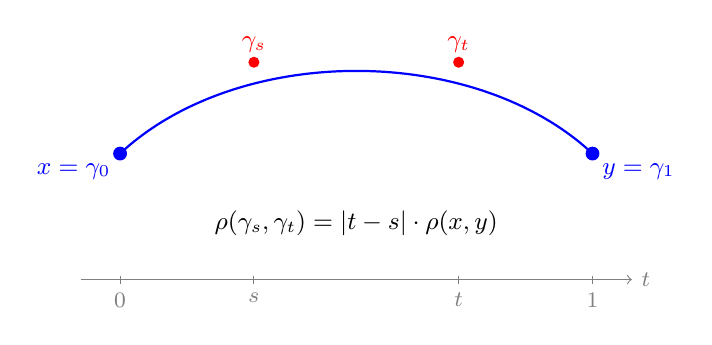
\begin{tikzpicture}[scale=1.0]
  %% 曲線（測地線 γ）
  \draw[thick, blue] (0, 0) .. controls (1.5, 1.4) and (4.5, 1.4) .. (6, 0);

  %% 端点と中間点
  \fill[blue] (0, 0) circle (2.5pt) node[below left, font=\small] {$x = \gamma_0$};
  \fill[blue] (6, 0) circle (2.5pt) node[below right, font=\small] {$y = \gamma_1$};

  %% 中間点 γ_s, γ_t
  \fill[red] (1.7, 1.16) circle (2pt) node[above, font=\small] {$\gamma_s$};
  \fill[red] (4.3, 1.16) circle (2pt) node[above, font=\small] {$\gamma_t$};

  %% 距離関係の式
  \node[font=\small, anchor=north] at (3.0, -0.6)
    {$\rho(\gamma_s, \gamma_t) = |t - s| \cdot \rho(x, y)$};

  %% 時間軸
  \draw[->, gray] (-0.5, -1.6) -- (6.5, -1.6) node[right, font=\footnotesize, gray] {$t$};
  \foreach \xpos/\lab in {0/0, 1.7/s, 4.3/t, 6/1} {
    \draw[gray] (\xpos, -1.55) -- (\xpos, -1.65);
    \node[gray, font=\footnotesize, below] at (\xpos, -1.65) {$\lab$};
  }
\end{tikzpicture}
\caption{距離空間 $(M, \rho)$ における定速測地線 $\gamma \colon [0, 1] \to M$
の概念図．$\rho(\gamma_s, \gamma_t)$ は時刻差 $|t - s|$ に
$\rho(x, y)$ を掛けただけの値となり，経路上の任意の 2 点間で
「直線的」な距離関係が成り立つ．}
\label{fig:sem-constant-geodesic}
\end{figure}

\subsection{本章を貫く問い}

\begin{memo*}
  以下，本章を貫く問いは次のものである：
  \begin{quote}
    基底空間 $(\X, d)$ が測地空間であるとき，
    Wasserstein 空間 $(\Pp_p(\X), \Wass_p)$ もまた測地空間か？\\
    そうであれば，$\Wass_p$-測地線は具体的にどのように与えられるか？
  \end{quote}
  この問いに肯定的に答えるのが次節の\textbf{変位補間}（McCann interpolation）
  であり，それは「最適カップリング上で各点ペアを基底空間の測地線で結ぶ」
  という非常に自然な構成によって与えられる．
\end{memo*}

%% ============================================================
%% §3 変位補間
%% ============================================================
\section{変位補間}
\label{sec:sem-displacement}

本節では，まず最も具体的な舞台 $\X = \R^n$, $p = 2$ で
変位補間（McCann 補間）を導入し，それが $\Wass_2$-測地線になることを示す．
最後に一般の Polish 測地空間への拡張について述べる．

\subsection{ユークリッド設定と Brenier の定理}

\begin{setting}{本節の設定（§3.1, §3.2）}{sem-displacement-setup}
  以下 §3.1, §3.2 では次の設定を採用する：
  \begin{itemize}
    \item $\X = \R^n$, 距離 $d(x, y) = \norm{x - y}_2$, 測度 $\Lcal^n$．
    \item $p = 2$，コスト $c(x, y) = \norm{x - y}_2^2$．
    \item $\alpha \in \Pp_2(\R^n)$ はルベーグ測度に関し絶対連続：
      $\alpha \ll \Lcal^n$．
    \item $\beta \in \Pp_2(\R^n)$（絶対連続性は要求しない）．
  \end{itemize}
  この設定では Brenier の定理（次の定理~\ref{thm:sem-brenier}）
  により Kantorovich 問題の最適解が「写像」の形に書ける．
\end{setting}

\begin{theorem}{Brenier の定理}{sem-brenier}
  設定~\ref{set:sem-displacement-setup} の下で，
  Kantorovich 問題（定義~\ref{def:sem-kantorovich}）には次が成立する：
  \begin{enumerate}
    \item[\textup{(1)}] 最適カップリング $\pi^* \in \Couplings(\alpha, \beta)$ は
      \textbf{一意}であり，ある可測写像 $T \colon \R^n \to \R^n$ により
      Monge 写像のグラフ上に集中する：
      $\pi^* = (\Id, T)\pushforward \alpha$．
      特に $T\pushforward \alpha = \beta$．
    \item[\textup{(2)}] さらに $T$ はある凸関数
      $\varphi \colon \R^n \to \R \cup \{+\infty\}$ の勾配として
      $T(x) = \nabla \varphi(x)$（$\alpha$-a.e.）と書ける．
    \item[\textup{(3)}] $\varphi$ は加法定数を除いて $\alpha$-a.e.\ 一意である．
  \end{enumerate}
\end{theorem}

本セミナーでは Brenier 定理の証明には立ち入らない．
証明には凸双対性（$c$-変換）と $\alpha \ll \Lcal^n$ の本質的活用が必要であり，
詳細は Cuturi 訳「Brenier の定理」節および Villani の教科書
\textit{Topics in Optimal Transportation} 等を参照されたい．

\begin{memo*}
  \textbf{Monge--Amp\`{e}re 方程式．}
  $\alpha, \beta$ がともに密度 $\rho_\alpha, \rho_\beta$ を持つとき，
  Brenier 定理の凸関数 $\varphi$ は
  \[
    \det\bigl( \partial^2 \varphi(x) \bigr) \,
    \rho_\beta\bigl( \nabla \varphi(x) \bigr) = \rho_\alpha(x)
  \]
  という非線形 PDE（Monge--Amp\`{e}re 方程式）を満たす．
  これは「凸関数 $\varphi$ の Hessian 行列式が密度比を再現する」という
  幾何的条件で，最適輸送と非線形 PDE 理論を結ぶ橋となっている．
\end{memo*}

\subsection{McCann の変位補間}

Brenier の定理が与える写像 $T = \nabla \varphi$ を用いると，
$\alpha$ から $\beta$ への「補間」を以下のように自然に定義できる．

\begin{definition}{変位補間（McCann interpolation）}{sem-displacement-interpolation}
  設定~\ref{set:sem-displacement-setup} の下で，Brenier 写像
  $T = \nabla \varphi$（定理~\ref{thm:sem-brenier}）を用い，
  各 $t \in [0, 1]$ に対して
  \[
    T_t \colon \R^n \to \R^n,\;
    T_t(x) \defeq (1 - t)\, x + t\, T(x)
  \]
  と定める．このとき
  \[
    \mu_t \defeq (T_t)\pushforward \alpha \in \Pp_2(\R^n)
    \qquad (t \in [0, 1])
  \]
  を $\alpha$ から $\beta$ への\textbf{変位補間}（McCann interpolation）と呼ぶ．
  両端は $\mu_0 = \alpha$，$\mu_1 = T\pushforward \alpha = \beta$．
\end{definition}

\begin{figure}[H]
\centering
\begin{tikzpicture}[scale=1.0]
  %% 3 段の密度カーブ：t = 0, 1/2, 1
  \foreach \tval/\xshift/\labpos/\lab in
    {0/0/-2.5/{$\mu_0 = \alpha$}, 0.5/5.0/-2.5/{$\mu_{1/2}$}, 1/10.0/-2.5/{$\mu_1 = \beta$}}
  {
    \begin{scope}[xshift=\xshift cm]
      %% 軸
      \draw[thick, ->] (-0.3, 0) -- (4.3, 0) node[right, font=\footnotesize] {};
      \draw[thick, ->] (0, -0.2) -- (0, 1.8);

      %% 2 つのガウシアン山（α, μ_t, β を変位で動かす）
      %% α: 中心 (1.0, 2.8), β: 中心 (3.0, 1.5), μ_t: 線形補間
      %% ここでは中心位置だけを変位補間して 2 山の山型を描く
      \pgfmathsetmacro{\cAa}{1.0 + \tval * 1.0}   % 第 1 山中心 x
      \pgfmathsetmacro{\cBb}{2.5 + \tval * 0.5}   % 第 2 山中心 x
      \pgfmathsetmacro{\hAa}{0.7 + \tval * 0.4}   % 第 1 山高さ
      \pgfmathsetmacro{\hBb}{1.0 - \tval * 0.3}   % 第 2 山高さ
      \draw[blue, thick, smooth, samples=80, domain=0:4]
        plot (\x, {\hAa * exp(-(\x - \cAa) * (\x - \cAa) * 5)
                   + \hBb * exp(-(\x - \cBb) * (\x - \cBb) * 6)});

      %% ラベル
      \node[font=\small, below] at (2.0, \labpos) {\lab};
      \node[font=\footnotesize, gray, above right] at (-0.1, 1.6) {密度};
    \end{scope}
  }

  %% 横の矢印（時間 t の流れ）
  \draw[->, very thick, gray] (4.7, 0.8) -- (5.3, 0.8);
  \draw[->, very thick, gray] (9.7, 0.8) -- (10.3, 0.8);

  %% 全体ラベル
  \node[font=\small, anchor=north] at (7.0, -3.2)
    {$\mu_t = ((1 - t)\Id + t T)\pushforward \alpha$,\quad
     $T = \nabla \varphi$ は Brenier 写像};
\end{tikzpicture}
\caption{$\R$ 上の 2 山測度に対する変位補間の概念図．
$t = 0$ で $\alpha$，$t = 1$ で $\beta$ となり，
中間時刻では各点が Brenier 写像 $T$ に向かって直線的に動く．
線形補間 $(1 - t)\alpha + t \beta$（質量の単純混合）とは異なり，
変位補間は\textbf{基底空間内で各点が動く}結果として得られる
ことに注意（質量の縦方向の高さ変化ではなく，横方向の移動）．}
\label{fig:sem-displacement-interpolation}
\end{figure}

\begin{theorem}{変位補間は $\Wass_2$-測地線である}{sem-displacement-geodesic}
  設定~\ref{set:sem-displacement-setup} の下で，
  変位補間 $\mu_t = (T_t)\pushforward \alpha$ は
  $(\Pp_2(\R^n), \Wass_2)$ における $\alpha$ から $\beta$ への定速測地線である．
  すなわち
  \[
    \Wass_2(\mu_s, \mu_t) = |t - s| \cdot \Wass_2(\alpha, \beta)
    \qquad (\forall\, s, t \in [0, 1]).
  \]
\end{theorem}

\begin{proof}
  $0 \leq s \leq t \leq 1$ として議論すれば十分である（一般の場合は対称性から従う）．

  \textbf{(a) 上界．}
  写像 $(T_s, T_t) \colon \R^n \to \R^n \times \R^n$ による
  $\alpha$ の押し出し
  \[
    \pi_{s, t} \defeq (T_s, T_t)\pushforward \alpha
    \in \Mm_+^1(\R^n \times \R^n)
  \]
  は $\Couplings(\mu_s, \mu_t)$ の元である．
  実際，$(P_1)\pushforward \pi_{s,t} = (T_s)\pushforward \alpha = \mu_s$，
  $(P_2)\pushforward \pi_{s,t} = (T_t)\pushforward \alpha = \mu_t$．
  これを Wasserstein 距離の評価に用いると
  \begin{align*}
    \Wass_2(\mu_s, \mu_t)^2
    &\leq \int_{\R^n \times \R^n} \norm{u - v}_2^2 \, \d\pi_{s, t}(u, v) \\
    &= \int_{\R^n} \norm{T_s(x) - T_t(x)}_2^2 \, \d\alpha(x) \\
    &= \int_{\R^n} \norm{(s - t)(x - T(x))}_2^2 \, \d\alpha(x) \\
    &= |t - s|^2 \int_{\R^n} \norm{x - T(x)}_2^2 \, \d\alpha(x) \\
    &= |t - s|^2 \cdot \Wass_2(\alpha, \beta)^2,
  \end{align*}
  最後の等式は $T = \nabla \varphi$ が最適カップリングを実現する
  Brenier 写像（定理~\ref{thm:sem-brenier}）であることによる．
  したがって $\Wass_2(\mu_s, \mu_t) \leq |t - s| \cdot \Wass_2(\alpha, \beta)$．

  \textbf{(b) 下界．}
  距離 $\Wass_2$ の三角不等式（定理~\ref{thm:sem-wass-metric}）を
  $\mu_0 = \alpha, \mu_s, \mu_t, \mu_1 = \beta$ に繰り返し適用すると
  \[
    \Wass_2(\alpha, \beta)
    \leq \Wass_2(\alpha, \mu_s) + \Wass_2(\mu_s, \mu_t) + \Wass_2(\mu_t, \beta).
  \]
  上界 (a) より右辺第 1 項 $\leq s \Wass_2(\alpha, \beta)$，
  第 3 項 $\leq (1 - t) \Wass_2(\alpha, \beta)$ なので
  \[
    \Wass_2(\alpha, \beta)
    \leq s \Wass_2(\alpha, \beta) + \Wass_2(\mu_s, \mu_t) + (1 - t) \Wass_2(\alpha, \beta)
  \]
  整理して
  $\Wass_2(\mu_s, \mu_t) \geq (t - s) \Wass_2(\alpha, \beta)
  = |t - s| \cdot \Wass_2(\alpha, \beta)$．

  (a) と (b) を合わせて等号を得る．
\end{proof}

\begin{example}{Dirac の変位補間}{sem-displacement-dirac}
  $\alpha = \delta_x, \beta = \delta_y$ の場合，
  正確には $\delta_x \not\ll \Lcal^n$ ゆえ Brenier の定理の前提を満たさないが，
  最適カップリングが $\pi^* = \delta_{(x, y)}$ で一意に与えられることは直接見られ，
  これは「写像 $T \equiv y$」のグラフへの集中とみなせる．
  したがって $T_t(x) = (1 - t) x + t y$ を採用すると，変位補間は
  \[
    \mu_t = (T_t)\pushforward \delta_x = \delta_{T_t(x)} = \delta_{(1 - t) x + t y}.
  \]
  例~\ref{ex:sem-geodesic-euclidean} で見た $\R^n$ の直線
  $\gamma_t = (1 - t) x + t y$ が，等長埋め込み
  $z \mapsto \delta_z$（例~\ref{ex:sem-wass-dirac}）の下で
  $\Wass_2$-測地線 $\delta_{\gamma_t}$ に持ち上がっている．
  「基底空間の測地線が測度空間の測地線を生成する」という構図の最も透明な例である．
\end{example}

\subsection{一般の Polish 空間への拡張}

\begin{remark}{一般化と限界}{sem-displacement-general}
  例~\ref{ex:sem-displacement-dirac} の観察を一般化すると，
  $\R^n$ という線形構造に頼らずとも，
  \textbf{基底空間 $(\X, d)$ が測地空間}（定義~\ref{def:sem-geodesic-space}）でさえあれば
  Wasserstein 空間にも測地線が構成できる．
  概略は以下である：
  \begin{enumerate}
    \item[\textup{(a)}]
      $\alpha, \beta \in \Pp_2(\X)$ に対する Kantorovich 問題に最適カップリング
      $\pi^* \in \Couplings(\alpha, \beta)$ を取る
      （Polish + コスト下半連続性の下で存在）．
    \item[\textup{(b)}]
      各ペア $(x, y) \in \X \times \X$ に $x$ から $y$ への定速測地線
      $\gamma^{x, y} \colon [0, 1] \to \X$ を可測に選択する（測地的選択）．
      $(x, y) \mapsto \gamma_t^{x, y}$ が可測となるよう選べることは，
      $\X$ が完備可分という Polish 性が必要となる箇所である．
    \item[\textup{(c)}]
      評価写像 $e_t(x, y) \defeq \gamma_t^{x, y}$（時刻 $t$ の点を返す写像）
      による押し出し
      \[
        \mu_t \defeq (e_t)\pushforward \pi^* \in \Pp_2(\X)
      \]
      が $\alpha$ から $\beta$ への $\Wass_2$-測地線となる．
  \end{enumerate}
  ユークリッド設定（設定~\ref{set:sem-displacement-setup}）はこの一般構成で
  $\gamma_t^{x, y} = (1 - t) x + t y$（直線），
  $\pi^* = (\Id, T)\pushforward \alpha$（Brenier 写像のグラフ）と
  特殊化したものに他ならない．証明と詳細は Ambrosio--Gigli--Savar\'{e}
  \textit{Gradient Flows in Metric Spaces and in the Space of Probability Measures}，
  Villani \textit{Optimal Transport: Old and New} を参照．
\end{remark}

\begin{theorem}{基底測地空間の Wasserstein 空間は測地空間}{sem-wass-geodesic-space}
  $(\X, d)$ を Polish 距離測地空間とすると，
  $(\Pp_2(\X), \Wass_2)$ もまた測地空間である．
  すなわち任意の $\alpha, \beta \in \Pp_2(\X)$ に対し，
  $\alpha$ から $\beta$ への $\Wass_2$-定速測地線
  $(\mu_t)_{t \in [0, 1]}$ が少なくとも 1 つ存在する．
\end{theorem}

これにより §2.3 の問い（基底が測地空間ならば Wasserstein 空間も測地空間か？）
には肯定的に答えられた．
ユークリッド設定（定理~\ref{thm:sem-displacement-geodesic}）と
Dirac の例（例~\ref{ex:sem-displacement-dirac}）から窺われるように，
Wasserstein 空間の測地線は「質量の混合（線形補間）」ではなく
「質量の移動（変位補間）」によって与えられる．これは次節以降の
「Wasserstein 空間は Riemann 多様体的な構造を持つ」という直感を支える事実である．

%% ============================================================
%% §4 Wasserstein 空間の幾何（直感）
%% ============================================================
\section{Wasserstein 空間の幾何}
\label{sec:sem-otto}

前節で $(\Pp_2(\R^n), \Wass_2)$ が測地空間であり，測地線は変位補間で与えられる
ことを見た．本節ではこの空間に対する 2 つの「幾何的」視点を導入する：
動的定式化（Benamou--Brenier）と，Otto による無限次元 Riemann 多様体の heuristics．
両者とも厳密な定式化は本セミナーの範囲を超えるが，§5 の曲率の議論への動機付けとして
押さえておく価値がある．

\subsection{Benamou--Brenier の動的定式化}

\begin{proposition}{Benamou--Brenier の動的定式化}{sem-benamou-brenier}
  $\alpha, \beta \in \Pp_2(\R^n)$ がともに密度 $\rho_\alpha, \rho_\beta$ を持つとき，
  \[
    \Wass_2(\alpha, \beta)^2
    = \inf_{(\rho, v)}
    \int_0^1 \int_{\R^n} \norm{v_t(x)}_2^2 \, \rho_t(x) \, \d x \, \d t
  \]
  ここで下限は，連続方程式
  \[
    \partial_t \rho_t + \nabla \cdot (\rho_t v_t) = 0
    \qquad (t \in (0, 1))
  \]
  を弱解の意味で満たし，かつ境界条件 $\rho_0 = \rho_\alpha$, $\rho_1 = \rho_\beta$
  を満たす全ての時間依存密度 $\rho \colon [0, 1] \to L^1_+(\R^n)$ と
  時間依存ベクトル場 $v \colon [0, 1] \to \mathrm{Vec}(\R^n)$ の組 $(\rho, v)$
  にわたる．
\end{proposition}

証明と厳密な定式化は Benamou--Brenier (2000) 原論文を参照．

\begin{memo*}
  \textbf{流体力学的解釈．}
  Benamou--Brenier 定式化は次のように読める：
  「$\Wass_2(\alpha, \beta)^2$ は，密度 $\rho_t$ をもつ流体を
  時刻 0 で $\alpha$，時刻 1 で $\beta$ となるよう連続方程式に従って動かす
  際の，運動エネルギー総積分
  $\int_0^1 \int \frac{1}{2} \norm{v_t}^2 \rho_t \, \d x \, \d t$ の最小値の
  2 倍に等しい．」
  つまり Wasserstein 距離は，質量を「掘り起こして瞬間移動させる」のではなく
  「速度場で連続的に流す」運動コストとして特徴づけられる．
  この視点は次の Otto 計算への自然な橋となる．
\end{memo*}

\subsection{Otto の Riemann 構造（heuristics）}

\begin{memo*}
  \textbf{Otto 計算（formal な Riemann 構造）．}
  $P_2 = \Pp_2(\R^n)$ を「無限次元 Riemann 多様体」と見なす Otto の構成
  （Otto 2001，Jordan--Kinderlehrer--Otto 1998）を概略する：
  \begin{enumerate}
    \item[\textup{(i)}] 接空間．$\mu \in P_2$（密度 $\rho > 0$）における接空間を，
      連続方程式 $\partial_t \mu + \nabla \cdot (\mu v) = 0$ の許容速度場 $v$
      の同値類とみなす．これは $L^2(\mu)$ における勾配場の閉包
      \[
        \Tan_\mu P_2
        \simeq \overline{\{\nabla \phi \mid \phi \in C^\infty_c(\R^n)\}}^{L^2(\mu)}
      \]
      と同型．
    \item[\textup{(ii)}] Riemann 計量．接ベクトル
      $\nabla \phi, \nabla \psi \in \Tan_\mu P_2$ に対する内積を
      \[
        \langle \nabla \phi, \nabla \psi \rangle_\mu
        \defeq \int_{\R^n} \langle \nabla \phi(x), \nabla \psi(x) \rangle \, \d\mu(x)
      \]
      で定める．
    \item[\textup{(iii)}] 測地線．この Riemann 構造の下で測地線方程式の解は
      ちょうど McCann の変位補間（定義~\ref{def:sem-displacement-interpolation}）
      に一致する．
    \item[\textup{(iv)}] 勾配流．汎関数 $F \colon P_2 \to \R$ に対する
      Wasserstein 勾配流は $\partial_t \mu_t = \nabla \cdot (\mu_t \nabla \delta F / \delta \mu)$
      の形をとる．特に \textbf{相対エントロピー
      $\Hm(\mu \mid \Lcal^n) = \int \rho \log \rho \, \d x$ の Wasserstein 勾配流は
      熱方程式}（Jordan--Kinderlehrer--Otto 1998）：
      \[
        \partial_t \rho_t = \Delta \rho_t.
      \]
  \end{enumerate}
  これらは厳密な無限次元微分幾何としては正当化に技術的工夫
  （絶対連続曲線・metric derivative・$|\partial F|$ など）を要するが，
  「$P_2$ は無限次元 Riemann 多様体的な構造を持ち，その上で
  自然な汎関数（相対エントロピー）の勾配流が古典的 PDE（熱方程式）に一致する」
  という像が，§5 の曲率定義の背骨となる．
\end{memo*}

%% ============================================================
%% §5 曲率の下界
%% ============================================================
\section{曲率の下界（測地的凸性による特徴づけ）}
\label{sec:sem-curvature}

これまでに $(\Pp_2(\X), \Wass_2)$ が距離空間（§1），測地空間（§3），
さらに heuristics として Riemann 多様体的な構造（§4）を持つことを見た．
この最後の構造に注目すると，「曲率」を定義することができる．
Riemann 多様体 $(M, g)$ における Ricci 曲率を，
$(\Pp_2(M), \Wass_2)$ 上の関数（相対エントロピー）の凸性として書き換えるのが
\textbf{Sturm--von Renesse の同値定理}であり，
それを足場に距離測度空間一般へ拡張するのが Lott--Sturm--Villani の
$\CD(K, \infty)$ 条件である．

\begin{memo*}
  \textbf{Riemann 幾何の Ricci 曲率．}
  Riemann 多様体 $(M, g)$ 上の Ricci 曲率テンソル $\Ric_g$ は，
  接空間上の対称双線形形式（一階の曲率不変量）であり，次のような幾何的役割を担う：
  \begin{itemize}
    \item 体積要素の比較（Bishop--Gromov）
    \item 平行な測地線束の発散・収束（Jacobi 場）
    \item 熱核の long-time 挙動
  \end{itemize}
  「点ごとに最小固有値が $K$ 以上」（$\Ric_g \geq K g$）という条件は，
  $K > 0$ なら球面的な収束（Bonnet--Myers），
  $K = 0$ ならユークリッド的，
  $K < 0$ なら双曲的傾向，という定性的描像を与える．
\end{memo*}

\subsection{相対エントロピーと変位凸性}

\begin{definition}{相対エントロピー}{sem-relative-entropy}
  $\X$ 上に基準測度 $m$（典型的には Riemann 多様体上の体積測度 $\mathrm{vol}_g$，
  あるいは $\R^n$ 上のルベーグ測度 $\Lcal^n$）が与えられているとき，
  $\mu \in \Pp_2(\X)$ に対する $m$ に関する\textbf{相対エントロピー}を
  \[
    \Hm(\mu \mid m) \defeq
    \begin{cases}
      \displaystyle \int_{\X} \rho \log \rho \, \d m
      & \text{if } \mu = \rho \cdot m \;(\text{密度 } \rho \text{ をもつ}), \\[1ex]
      +\infty & \text{otherwise.}
    \end{cases}
  \]
  と定める．
\end{definition}

\begin{definition}{$K$-変位凸性}{sem-K-displacement-convex}
  汎関数 $F \colon \Pp_2(\X) \to \R \cup \{+\infty\}$ と
  実数 $K \in \R$ に対し，
  $F$ が\textbf{$K$-変位凸}（$K$-displacement convex）であるとは，
  任意の $\mu_0, \mu_1 \in \Pp_2(\X)$ と任意の $\Wass_2$-定速測地線
  $(\mu_t)_{t \in [0, 1]}$（定義~\ref{def:sem-constant-geodesic} を
  $(\Pp_2(\X), \Wass_2)$ に適用したもの）について
  \[
    F(\mu_t) \leq (1 - t)\, F(\mu_0) + t\, F(\mu_1)
    - \frac{K}{2}\, t(1 - t)\, \Wass_2(\mu_0, \mu_1)^2
    \qquad (\forall\, t \in [0, 1])
  \]
  が成り立つことをいう．$K = 0$ は通常の凸性，$K > 0$ は強凸性に対応する．
\end{definition}

\begin{figure}[H]
\centering
\begin{tikzpicture}[scale=1.0]
  %% 軸
  \draw[thick, ->] (-0.3, 0) -- (5.5, 0) node[right, font=\small] {$t$};
  \draw[thick, ->] (0, -0.3) -- (0, 3.6) node[above, font=\small] {$F(\mu_t)$};

  %% 端点
  \fill (0, 2.5) circle (2pt);
  \fill (5, 2.5) circle (2pt);
  \node[font=\footnotesize, anchor=east] at (-0.05, 2.5) {$F(\mu_0)$};
  \node[font=\footnotesize, anchor=west] at (5.05, 2.5) {$F(\mu_1)$};

  %% 線形補間（破線）：(1-t)F(μ_0) + t F(μ_1)
  \draw[dashed, gray] (0, 2.5) -- (5, 2.5);
  \node[gray, font=\footnotesize, anchor=south] at (2.5, 2.55)
    {$(1 - t) F(\mu_0) + t F(\mu_1)$};

  %% K = 0（凸）：放物線が線形補間と一致 or 下に
  \draw[blue, thick, smooth, samples=80, domain=0:5]
    plot (\x, {2.5});
  \node[blue, font=\footnotesize, anchor=west] at (5.1, 2.0) {$K = 0$};

  %% K > 0（強凸）：下に強く出る放物線
  %% F(μ_t) ≤ (1-t)F(μ_0) + tF(μ_1) - (K/2) t(1-t) W^2
  \draw[red, thick, smooth, samples=80, domain=0:5]
    plot (\x, {2.5 - 0.6 * (\x / 5) * (1 - \x / 5) * 5});
  \node[red, font=\footnotesize, anchor=west] at (5.1, 1.4) {$K > 0$ (強凸)};

  %% K < 0（凸でない場合あり）：上に膨らむ
  \draw[orange, thick, smooth, samples=80, domain=0:5]
    plot (\x, {2.5 + 0.5 * (\x / 5) * (1 - \x / 5) * 5});
  \node[orange, font=\footnotesize, anchor=west] at (5.1, 3.0) {$K < 0$};

  %% 補助：t = 1/2 の縦線
  \draw[dotted, gray] (2.5, 0) -- (2.5, 3.2);
  \node[gray, font=\scriptsize, below] at (2.5, -0.05) {$t = 1/2$};
\end{tikzpicture}
\caption{$K$-変位凸性の概念図．横軸は $\Wass_2$-測地線上の時刻 $t$，
縦軸は汎関数 $F(\mu_t)$．灰色の破線は線形補間
$(1 - t) F(\mu_0) + t F(\mu_1)$．
$K = 0$ では $F(\mu_t)$ は線形補間以下（通常の凸性），
$K > 0$ ではさらに $\frac{K}{2} t(1 - t) \Wass_2^2$ だけ下にある（強凸），
$K < 0$ では上方への膨らみを許す．}
\label{fig:sem-displacement-convexity}
\end{figure}

\subsection{Sturm--von Renesse の同値定理と $\CD(K, \infty)$ 条件}

\begin{theorem}{Sturm--von Renesse の同値定理}{sem-sturm-renesse}
  $(M, g)$ を完備連結 Riemann 多様体，$\mathrm{vol}_g$ をその体積測度，
  $K \in \R$ とする．次の 2 条件は同値である：
  \begin{enumerate}
    \item[\textup{(a)}] 任意の点 $x \in M$ で $\Ric_g(x) \geq K g(x)$
      （Ricci テンソルが $K g$ 以上，最小固有値で評価）．
    \item[\textup{(b)}] 相対エントロピー $\Hm(\cdot \mid \mathrm{vol}_g)$ は
      $(\Pp_2(M), \Wass_2)$ 上で $K$-変位凸
      （定義~\ref{def:sem-K-displacement-convex}）．
  \end{enumerate}
\end{theorem}

これは Sturm--von Renesse (2005) の主結果である．
証明には Otto--Villani の HWI 不等式や Lichnerowicz 型の不等式，
測地線解析を要するため，ここでは省略する．

定理~\ref{thm:sem-sturm-renesse} の意義は次の点にある：
左辺 (a) は\textbf{微分幾何の局所量}（テンソル $\Ric_g$）であり，
右辺 (b) は\textbf{測度論的な大域量}（汎関数の凸性）である．
この同値性により，Riemann 構造を経由せず\textbf{距離と測度のみ}から
Ricci 下界を定義することが可能になる：

\begin{definition}{$\CD(K, \infty)$ 空間}{sem-cd-kinfty}
  距離測度空間 $(\X, d, m)$ が\textbf{$\CD(K, \infty)$ 条件}を満たすとは，
  $(\X, d)$ が Polish 距離測地空間であって，
  相対エントロピー $\Hm(\cdot \mid m) \colon \Pp_2(\X) \to \R \cup \{+\infty\}$
  が $K$-変位凸（定義~\ref{def:sem-K-displacement-convex}）であることをいう．
\end{definition}

定理~\ref{thm:sem-sturm-renesse} により，Riemann 多様体 $(M, g, \mathrm{vol}_g)$ の
$\CD(K, \infty)$ 性は古典的な $\Ric_g \geq K$ と一致する．
すなわち $\CD(K, \infty)$ は\textbf{Ricci 下界の同定義}である．

\subsection{例}

\begin{example}{ユークリッド空間：$K = 0$}{sem-cd-euclidean}
  $(\R^n, \norm{\cdot}_2, \Lcal^n)$ は $\CD(0, \infty)$ を満たす：
  相対エントロピー $\Hm(\cdot \mid \Lcal^n)$ は
  $(\Pp_2(\R^n), \Wass_2)$ 上で（通常の意味で）変位凸である．
  これは McCann (1997) によって最初に証明された displacement convexity の
  原型例である．Riemann 幾何側の $\Ric \equiv 0$（ユークリッド空間は曲率 0）と
  整合する．
\end{example}

\begin{example}{単位球面：$K = n - 1$}{sem-cd-sphere}
  $n$-次元単位球面 $S^n \subset \R^{n+1}$ に内在距離（大円距離）と
  正規化された体積測度を入れた空間は，$\Ric = (n - 1) g$ を持つ．
  したがって定理~\ref{thm:sem-sturm-renesse} より
  $S^n$ は $\CD(n - 1, \infty)$ を満たす．次元 $n$ が大きいほど Ricci 曲率の
  下界 $K = n - 1$ も大きくなる．
\end{example}

\begin{memo*}
  \textbf{$\CD(K, N)$ への発展．}
  $\CD(K, \infty)$ 条件は次元の情報を含まないため，
  例~\ref{ex:sem-cd-sphere} のように $K = n - 1$ という形で次元が現れても
  「次元上界」としては機能しない．
  この欠落を補うため，Lott--Sturm--Villani は Rényi エントロピー族
  $S_N(\mu \mid m) = -\int \rho^{1 - 1/N} \, \d m$ の変位凸性で次元上界 $N$ を組み込んだ
  $\CD(K, N)$ 条件を導入した．これにより
  Bishop--Gromov 体積比較や Bonnet--Myers 直径評価といった
  より精密な Riemann 幾何的結果が距離測度空間に持ち上がる．
  詳細は Villani \textit{Optimal Transport: Old and New} 第 14 章以降を参照．
\end{memo*}

\subsection{本章のメッセージ}

\begin{memo*}
  Kantorovich 問題（定義~\ref{def:sem-kantorovich}）はもともと，
  二つの確率測度 $\alpha, \beta$ を結ぶ「最適なカップリングを探す」最適化問題であった．
  本章ではコストを基底距離の $p$ 乗に特殊化することで，
  Kantorovich 最適値が確率測度空間 $\Pp_p(\X)$ 上の\textbf{距離} $\Wass_p$ となり
  （§1），その距離は\textbf{測地空間}の構造をもち（§3），
  測地線上で\textbf{相対エントロピーの凸性}を要求すると Riemann 幾何の
  \textbf{Ricci 下界} を測度論的に再定義できる（§5）ことを見た．
  最適輸送は単なる組合せ最適化を超えて，
  \textbf{確率測度の世界に微分幾何を持ち込む装置}として働く．
  この視座は，計算面でのアルゴリズム（第~\ref{ch:seminar-02}~章）と並ぶ，
  最適輸送理論のもう一つの大きな柱である．
\end{memo*}
